\documentclass[11pt]{article}
\usepackage[T1]{fontenc}
\usepackage[english]{babel}
\usepackage{csquotes}
\usepackage[margin=1in]{geometry}
\usepackage{amsmath, amssymb, amsthm}
\usepackage{graphicx}
\usepackage{booktabs}
\usepackage[style=numeric, sorting=none]{biblatex}
\addbibresource{references.bib}
\usepackage[colorlinks=true, allcolors=blue]{hyperref}

\newtheorem{theorem}{Theorem}
\newtheorem{lemma}[theorem]{Lemma}
\theoremstyle{definition}
\newtheorem{definition}[theorem]{Definition}

\title{{{TITLE}}}
\author{%
  {{AUTHOR}}\thanks{Department, Institution, City, Country.
    Email: \href{mailto:first.last@example.org}{first.last@example.org}.}%
}
\date{\today}

\begin{document}

\maketitle

\begin{abstract}
The abstract sets out in one paragraph the question studied, the method, the
main results and their significance. Most journals limit it to 150 or 250
words.

\medskip
\noindent\textbf{Keywords:} first keyword, second keyword, third keyword.
\end{abstract}

\section{Introduction}
\label{sec:introduction}

The introduction states the problem, sums up earlier work
\parencite{knuth1981, lamport1994} and announces the paper's contribution.
Section~\ref{sec:method} describes the method, Section~\ref{sec:results}
presents the results and Section~\ref{sec:conclusion} concludes.

\section{Method}
\label{sec:method}

\begin{definition}
A sequence $(u_n)$ of real numbers is \emph{bounded} if there is a real
number $M$ such that $\lvert u_n \rvert \le M$ for every integer $n$.
\end{definition}

\begin{theorem}[Bolzano--Weierstrass]
\label{thm:bw}
Every bounded real sequence has a convergent subsequence.
\end{theorem}

\begin{proof}
Split the interval $[-M, M]$ into two halves, one of which holds infinitely
many terms of the sequence, then start again within that half. The nested
intervals obtained in this way define the limit of a subsequence.
\end{proof}

The model studied is
\begin{equation}
  \label{eq:model}
  y_i = \beta_0 + \beta_1 x_i + \varepsilon_i, \qquad i = 1, \dots, n,
\end{equation}
where the errors $\varepsilon_i$ are independent with zero mean.

\section{Results}
\label{sec:results}

Table~\ref{tab:results} gives the estimated coefficients of
model~\eqref{eq:model} and Figure~\ref{fig:data} shows its fit.

\begin{table}[htbp]
  \centering
  \caption{Estimated coefficients.}
  \label{tab:results}
  \begin{tabular}{lrrr}
    \toprule
    Coefficient & Estimate & Std.\ error & $p$-value \\
    \midrule
    $\beta_0$ & 1.24 & 0.31 & $< 0.001$ \\
    $\beta_1$ & 0.87 & 0.12 & $< 0.001$ \\
    \bottomrule
  \end{tabular}
\end{table}

\begin{figure}[htbp]
  \centering
  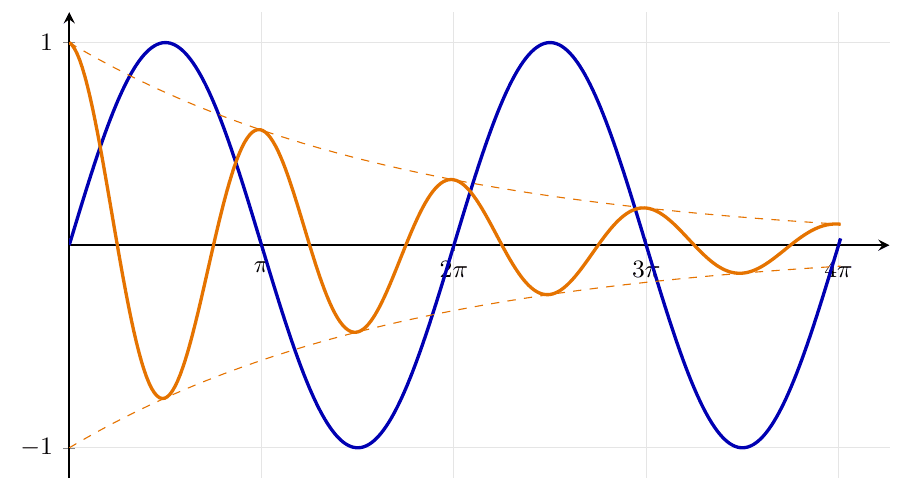
\includegraphics[width=0.7\linewidth]{images/curves.png}
  \caption{An image of the project: replace it with your own.}
  \label{fig:data}
\end{figure}

\section{Conclusion}
\label{sec:conclusion}

The conclusion recalls the results and looks ahead to future work
\parencite{mittelbach2023}.

\section*{Acknowledgments}

The authors thank the agencies that funded this work.

\printbibliography

\end{document}
